\section{Query Implementation}
In this section, we elaborate how we have implemented the query logic to achieve O(log n) time complexity. The 2015 Grand Challenge problem has two queries. First is to evaluate top ten most frequent routes within the last 30 minutes and second is to evaluate top ten profitable areas within the last 15 minutes. We can use composite objects to manage details for each route and cell and compare them to find top 10 values. However, each time window can have thousands of route and cell details. Therefore, an efficient data structure is needed to add, remove, update and retrieve top ten values from a set of objects for a given time window efficiently. Since each event is received with route and cell details, the aforementioned operations should be performed using route and cell details as the key. In order to support all these functions with O(log n) time complexity we have developed a data structure called \textit{NodeList}. The remainder of this section describes how we have achieved this time complexity with the \textit{NodeList} data structure and how we implemented queries using that data structure.

\subsection{NodeList Data Structure}

\begin{table}
\centering
\caption{Operations of \textit{NodeList} Data Structure}
\begin{tabular}{|l|l|} \hline
Operation Signature & Time Complexity \\ \hline \hline
add(key : Object, value : NodeValue) & O(log n) \\ \hline 
get(key : Object) : NodeValue & O(1) \\ \hline
containsKey(key : Object) : boolean & O(1) \\ \hline
remove(key : Object) : NodeValue & O(log n) \\ \hline
decrementPosition(key : Object) & O(log n) \\ \hline
incrementPosition(key : Object) & O(log n) \\ \hline
getTopValues() : List<NodeValue> & O(1) \\ \hline
\end{tabular}
\label{nodelist_api}
\end{table}

Table \ref{nodelist_api} shows the operations of this data structure. The \textit{NodeValue} is an interface to plug any user defined type as a value. For an example, the route query can use a \textit{RouteCount} object to keep route count while profitable cells query can use \textit{CellProfit} object to keep track of fare details. This interface contains a method called \texttt{compare} to define the order of the values. The \textit{NodeList} data structure provides the notion of a sorted values starting from position 0 (highest value) to its users. The \texttt{decrementPostion} operation moves the corresponding value towards position 0 until the correct position according to sorted order. Therefore this method should be called after increasing the value of an existing object. Similarly \texttt{incrementPosition} operation can be used to move a value to correct position after decreasing the value of an existing object. \texttt{GetTopValues} operation returns the top ten values of the list. The query algorithm sections further elaborate on the usage of these methods.

One way of implementing this data structure is to use a heap. A heap supports adding and extracting maximum value operations in O(log n) time. However, since this application requires top 10 values, we need to retrieve maximum value ten times and insert them back. On the other hand if we use a doubly linked list to store values, it will take O(n) time for  \texttt{decrementPostion} and \texttt{incrementPosition} operations. Therefore we can use a doubly linked list to keep first 10 values (this makes time complexity for all operations with this data structure O(1)) and a heap to keep other values to avoid above problems.  

The \textit{NodeList} data structure uses two data structures called \textit{OrderedList} to keep first 10 values and \textit{DynamicHeap} to keep other values. In this way it has to change only the last value of \textit{OrderedList} and maximum value of \textit{DynamicHeap} as required. Following sections describes how these data structures have been implemented with their operations.

\subsection{OrderedList Data Structure}

\begin{table}
\centering
\caption{Operations of \textit{OrderedList} Data Structure}
\begin{tabular}{|l|l|} \hline
Operation Signature & Time Complexity \\ \hline \hline
add(key : Object, value : NodeValue) & O(n) \\ \hline
containsKey(key : Object) : boolean & O(1) \\ \hline
get(key : Object) : NodeValue & O(1) \\ \hline
incrementPosition(key : Object) & O(n) \\ \hline
decrementPosition(key : Object) & O(n) \\ \hline
remove(key : Object) : NodeValue & O(1) \\ \hline
getLastPosition() : int & O(1) \\ \hline
getLastKey() : Object & O(1) \\ \hline
\end{tabular}
\label{orderedlist_api}
\end{table}

Table \ref{orderedlist_api} shows the operations of the \textit{OrderedList} data structure. First six methods have the same meaning as the \textit{NodeList} data structure and last two can be used to get the size of the list and the value of the last object. We internally keep a counter and a pointer to tail to support these operations in O(1) time. Figure \ref{orderedlist_impl} shows the implementation details. The \textit{Map} structure (an \textit{java.util.HashMap}) is used to retrieve object pointers with O(1) expected time. Each node of the doubly linked list points to previous and next nodes while storing the \textit{NodeValue}.


\begin{figure}[!t]
        \centering
        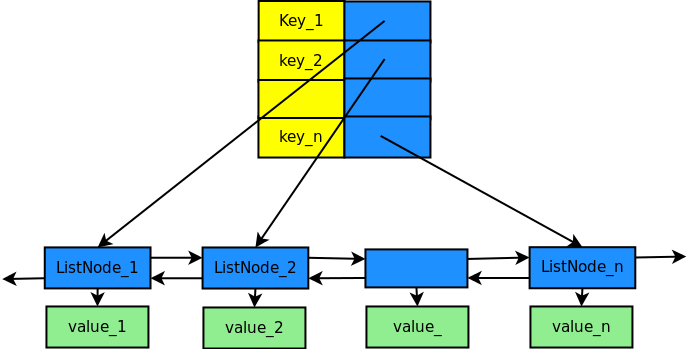
\includegraphics[width=3.0in]{orderedlist.png}
        \caption {A schematic representation of the \textit{OrderedList} data structure}
        \label{orderedlist_impl}
\end{figure}

\subsection{DynamicHeap Data Structure}

\begin{table}
\centering
\caption{Operations of \textit{DynamicHeap} Data Structure}
\begin{tabular}{|l|l|} \hline
Operation Signature & Time Complexity \\ \hline \hline
add(key : Object, value : NodeValue) & O(log n) \\ \hline
remove(key : Object) : NodeValue & O(log n) \\ \hline
containsKey(key : Object) : boolean & O(1) \\ \hline
get(key : Object) : NodeValue & O(1) \\ \hline
moveUp(key : Object) & O(log n) \\ \hline
moveDown(key : Object) & O(log n) \\ \hline
getMaxkey() : Object & O(1) \\ \hline
extractMax() : NodeValue & O(log n) \\ \hline
\end{tabular}
\label{dynamicheap_api}
\end{table}

Table \ref{dynamicheap_api} shows the operations of the \textit{DynamicHeap} data structure. \texttt{MoveUp} and \texttt{moveDown} operations are used to move an element up in the heap if the value increased, or move down in the heap if the value decreased. Figure \ref{dynamicheap_impl} shows the implementation details. Conventional heaps only support \texttt{add} and \texttt{extractMax} operations since heap operations require knowing the position of the element in underlying array. In order to support \texttt{moveUp}, \texttt{moveDown} and \texttt{remove} operations, we keep the array index with the object itself. As shown in figure \ref{dynamicheap_impl} \textit{HeapNode} object contains the array index and the \textit{NodeValue} given by the user. This allows us to retrieve array index in O(1) time and move the element O(log n) time.


\begin{figure}[!t]
        \centering
        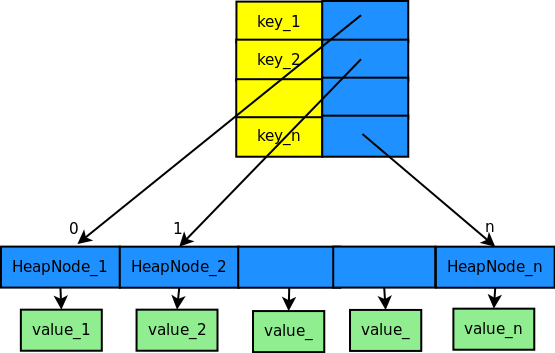
\includegraphics[width=3.0in]{DinamicHeap.png}
        \caption {A schematic representation of the \textit{DynamicHeap} data structure}
        \label{dynamicheap_impl}
\end{figure}

\subsection{Finding the Runing Median}
In general, we can find the runing median using two heaps. One to keep values greater than the current median and one to keep values less than the current median. An implementation of this algorithm using two \textit{java.util.PriorityQueue}s have an O(log n) time complexity for add operation and O(n) time complexity for remove operation (\texttt{remove} operation of \textit{java.util.PriorityQueue} takes O(n) time).  We overcame this issue using \textit{DynamicHeap} to keep values. In our solution, we use value as the key to insert and delete from the \textit{DynamicHeap} and keep each value with its count (same value can be repeated) in the \textit{DynamicHeap}. In the worst case this has a O(log n) time complexity for both the add and remove operations and in the best case (i.e value is already present and it does not cause a median change) it has O(1) time complexity.

\subsection{Frequent Routes Query}

The frequent routes query entails finding the most frequent routes within the last 30 minutes. Algorithm \ref{frequent_route_algorithm} shows the algorithm to process this query using the \textit{NodeList} data structure and a queue to keep the events for the time window.  Since queue operations are supported in O(1) time, query evaluations happen in O(log n) time. Algorithm \ref{frequent_route_algorithm} shows the basic algorithm to evaluate the query for an event. This algorithm assumes there is a global \textit{NodeList} object and route counts are stored in an object called \textit{RouteCount}. 

\begin{algorithm}
\caption{Algorithm to generate top 10 frequent route change events}
\label{frequent_route_algorithm}
\begin{algorithmic}
\small 
\STATE beforeTopTen $\leftarrow$ nodeList.getTopValues() 
\STATE window.add(event) 
\IF{ nodeList.containsKey(event.route) }
	\STATE routCount $\leftarrow$ nodeList.get(event.route) 
	\STATE routCount.count++ 
	\STATE nodeList.decrementPosition(event.route) 
\ELSE
	\STATE nodeList.add(event.route, new RouteCount(1)) 
\ENDIF

\WHILE{ there exists expired events }
	\STATE  expEvent $\leftarrow$ window.poll() 
	\STATE  routCount $\leftarrow$ nodeList.get(expEvent.route)
	\STATE  routCount.count-- 
	\IF{ routCount.count is 0 }
		\STATE nodelist.remove(expEvent.route)
	\ELSE
		\STATE nodeList.incrementPosition(expEvent.route) 
	\ENDIF
\ENDWHILE

\STATE nowTopTen $\leftarrow$ nodeList.getTopValues() 

\IF{ preTopTen not equals nowTopTen }
	\STATE create new event with top ten route details 
\ENDIF

\end{algorithmic}
\end{algorithm}

Each query evaluation can cause add, remove or update values of the existing time window objects. Therefore query processing mainly involves performing the above operations with the underlying \textit{NodeList} data structure and comparing top ten routes before and after. As shown in Algorithm \ref{frequent_route_algorithm}, when an event arrives, first it puts the event to time window to keep track for last 30 minutes. Then it adds new route value or updates the existing value and moves its position. Similarly, for expired events either it removes the values or reduces the count for existing values. Finally, two lists are compared to decide whether to generate an event or not. Here we have given a rough outline of the algorithm. Real implementation considers other factors such as sequence number to order events.

\subsection{Profitable Cells Query}

We have implemented profitable cells query in a similar manner to the frequent route query using  time windows. Complexity of the query raised following issues and we have solved them as given below.
\begin{enumerate}
	\item Profitability is calculated using the median profit and the number of empty taxis. In order to calculate the median, we use \textit{java.util.PriorityQueue} based approach mentioned in (Section 2.4). We choose this option over our implementation, because this approach performs better with smaller window sizes. First, these heap sizes do not grow over 145 and there are same values repeating in the list increasing the probability of finding a value without traversing the whole list. Secondly, our implementation creates more objects per operation compared to just keeping double values though the time complexity is O(log n). In section 4.3 we show that our approach works better for larger window sizes.
	\item In order to keep track of empty taxis, we need to process both pickup cell and dropoff cell details for each message. One way of doing this is to send all events for the same process instance and process both details with one event. However, this avoids the possibility of partitioning data across different processes. We generate two events, one for pickup data and one for dropoff data to make the process parallel. 
	\item In order to handle expiration of dropoff events, we keep track of the taxi ids currently available in a particular cell. If a pickup event occurs before dropoff event expiration, then we remove that taxi id from that cell and reduce the empty taxi count. In such a case, dropoff event expiration does not cause a reduction of taxi count.
\end{enumerate}

Algorithm \ref{pickup_algorithm} shows the logic to process pickup data. When a taxi gets a pickup, the taxi fare is added to that cell. We use \textit{ProfitCellNode} to keep the fare and empty taxi details to calculate the profitability. Then if its' taxi dropoff event has not been occurred (i.e this taxi has come to this location less than 30 minutes ago) it removes the taxi from that location. When the event get expired, it removes the fare from the \textit{ProfitCellNode}. 

\begin{algorithm}
\caption{Algorithm to process pickup data}
\label{pickup_algorithm}
\begin{algorithmic}
\small
\STATE beforeTopTen $ \leftarrow $ nodeList.getTopValues()
\STATE paymentWindow.add(event)
\IF {nodeList.containsKey(event.pickUpCell)}
	\STATE profitCellNode $ \leftarrow $ nodeList.get(event.pickUpCell)
	\STATE profitCellNode.addFare(event.fare)
	\IF {profitCellNode.containsTaxi(event.medalliion)}
		\STATE profitCellNode.emptyTaxi--
		\STATE profitCellNode.removeTaxi(event.medallion)
	\ENDIF
	\IF {profitablity has increased}
		\STATE nodeList.decrementPosition(event.pickUpCell)
	\ELSE
		\STATE nodeList.incrementPosition(event.pickUpCell)	
	\ENDIF
\ELSE
	\STATE nodeList.add(event.pickUpCell, new ProfitCellNode(event.fare))
\ENDIF
\WHILE {there exits expired events}
	\STATE expiredEvent $ \leftarrow $ paymentWindow.poll()
	\STATE profitCellNode $ \leftarrow $ nodeList.get(expiredEvent.pickUpCell)
	\STATE profitCellNode.removeFare(expiredEvent.fare)
	
	\IF {profitCellNode is empty}
		\STATE nodeList.remove(expiredEvent.pickUpCell)
	\ELSIF {profitablity increased}
		\STATE nodeList.decrementPosition(event.pickUpCell)
	\ELSE
		\STATE nodeList.incrementPosition(event.pickUpCell)
	\ENDIF
\ENDWHILE
\STATE nowTopTen $ \leftarrow $ nodeList.getTopValues()
\IF {beforeTopTen not equals to nowTopTen}
	\STATE emit a top ten change event
\ENDIF		 

\end{algorithmic}
\end{algorithm}

Algorithm \ref{dropoff_algorithm} shows the logic to process dropoff data. When a taxi trip ended in a location, number of empty taxis of that location has to be increased. If the taxi does not get a pickup within 30 mintes, then that taxi has to be removed from that location.

\begin{algorithm}
\caption{Algorithm to process dropoff data}
\label{dropoff_algorithm}
\begin{algorithmic}
\small
\STATE beforeTopTen $ \leftarrow $ nodeList.getTopValues()
\STATE dropWindow.add(event)
\IF {nodeList.containsKey(event.dropOffCell)}
	\STATE profitCellNode $ \leftarrow $ nodeList.get(event.dropOffCell)
	\STATE profitCellNode.addTaxi(event.medallion)
	\STATE profitCellNode.emptyTaxi++
	\STATE nodeList.incrementPosition(event.dropOffCell)	

\ELSE
	\STATE nodeList.add(event.dropOffCell, new ProfitCellNode(event.medallion))
\ENDIF
\WHILE {there are expired events}
	\STATE expiredEvent $ \leftarrow $ dropWindow.poll()
	\STATE profitCellNode $ \leftarrow $ nodeList.get(expiredEvent.dropOffCell)
	\IF {profitCellNode.containsTaxi(expiredEvent.medallion)}
		\STATE profitCellNode.emptyTaxi--
		\STATE profitCellNode.removeTaxi(expiredEvent.medallion)
		
		\IF {profitCellNode is empty}
			\STATE nodeList.remove(event.dropoffCell)
		\ELSE 
			\STATE nodeList.decrementPosition(event.dropOffCell) 
		\ENDIF
	\ENDIF
\ENDWHILE

\end{algorithmic}
\end{algorithm}





